\chapter{Problemanalyse}

\section{Problemstellung}

Das Projekt „Intelligentes Testen autonomer Fahrzeuge“ hat das Ziel, verifizier- und validierbare Tests für autonome Fahrsysteme (Automated Driving Systems, ADS) auf kostengünstige, reproduzierbare und skalierbare Weise bereitzustellen. Tests im realen Verkehr oder auf Teststrecken sind teuer, gefährlich und oft schlecht reproduzierbar. Deshalb müssen Tests zunehmend in virtuellen Umgebungen durchgeführt werden. Gleichzeitig sind Testfälle für ADS nicht nur einzelne, klar definierte Abläufe, sondern komplexe, parametrisierbare Szenarien mit dynamischen Akteuren (Fahrzeuge, Fußgänger, Wetter, Infrastruktur), was zu einer hohen Kombinatorik und schwer planbaren Ausführungen führt. Diese Kernprobleme gelten als Motivation für eine simulationsbasierte Testumgebung, um Ansätze für die Modellierung und Ausführung von Testszenarien zu erforschen. (vgl. \cite{EinfuehrungIntegrationsprojekt})

\section{Herausforderungen}

\begin{description}
    \item[Szenario-Komplexität und hohe Kombinationenvielfalt] Szenarien bestehen aus vielen Akteuren und parallelen Phasen. Die Anzahl möglicher Ausprägungen (Parameterkombinationen bzw. Reihenfolgen von Aktionen) ist sehr hoch, was eine systematische Abdeckung schwierig macht.(vgl. \cite{EinfuehrungIntegrationsprojekt})
    \item[Unvorhersehbares Verhalten des Vehicle-Under-Test (VUT).] Selbst bei korrekt spezifizierten Szenarien kann das VUT anders reagieren als erwartet. Dadurch entstehen zwei verschiedene Situationen, die getrennt voneinander betrachtet werden müssen: (a) Das Testziel konnte in einer Ausführung nicht erreicht werden (Szenario ist nicht erfüllbar) oder (b) das VUT verhält sich falsch (Testfehlverhalten). Diese Unterscheidung ist für die Auswertung und Weiterarbeit von zentraler Bedeutung.(vgl. \cite{EinfuehrungIntegrationsprojekt})
    \item[Semantische Lücken in Szenariensprachen] Viele formale Szenariobeschreibungen (z. B. OSC DSL) sind deklarativ und liefern keine operationale Semantik, sodass unklar ist, wie eine Ausführung Schritt für Schritt erzeugt werden kann. Deshalb sind Mechanismen erforderlich, die aus abstrakten, constraint-basierten Beschreibungen ausführbare Steuerungsbefehle generieren.(vgl. \cite{EinfuehrungIntegrationsprojekt})
    \item[Notwendigkeit intelligenter Ausführungsstrategien] Naive „Next-Step“-Heuristiken verletzen oft Constraints. Fortgeschrittene Verfahren wie Constraint-Solver, Reinforcement Learning (RL) oder evolutionäre Algorithmen können zwar bessere Ergebnisse liefern, sind aber meist rechenintensiv und benötigen viele Episoden bzw. Iterationen für das Training oder die Suche.(vgl. \cite{EinfuehrungIntegrationsprojekt})
    \item[Fehlende oder uneinheitliche Observability und Reporting] Für eine aussagekräftige Evaluation sind strukturierte Observation-Schnittstellen (z. B. Helper-Funktionen zum Abruf von Abständen, Spurfreigaben etc.) sowie umfassende Log-/Reporting-Mechanismen erforderlich, um Testziele und VUT-Reaktionen transparent auswerten zu können.(vgl. \cite{EinfuehrungIntegrationsprojekt})
\end{description}

\section{Use-Cases}

Um aus den identifizierten Problemen und Herausforderungen konkrete Anforderungen an die Testumgebung abzuleiten, ist es sinnvoll, typische Anwendungsszenarien zu betrachten. Diese Use Cases verdeutlichen, welche Nutzergruppen mit dem System interagieren und welche Ziele sie dabei verfolgen. So wird deutlich, wie die Testumgebung im praktischen Einsatz genutzt werden soll und welche Funktionalitäten sie mindestens bereitstellen muss.

\begin{figure}[h]
    \centering
    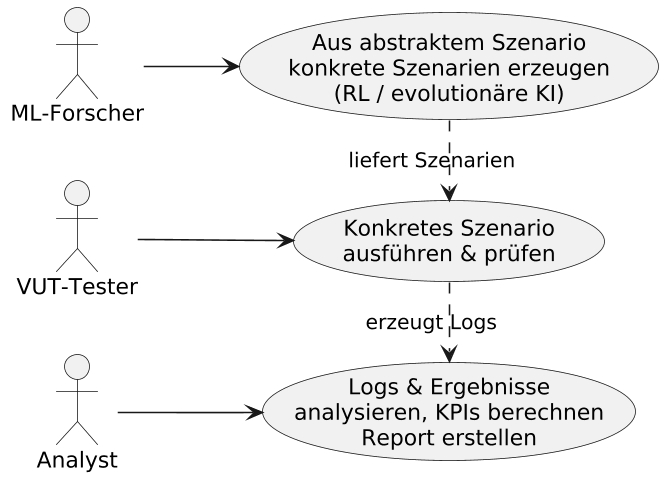
\includegraphics[width=0.5\textwidth]{contents/figures/UseCaseDiagramm_InteProjekt.png}
    \caption{Use-Case-Diagramm für die Testumgebung}
    \label{fig:UseCaseDiagramm}
\end{figure}


\begin{description}
    \item[VUT-Tester] Als Tester eines VUTs möchte ich konkrete Szenarien in der Testumgebung ausführen und anschließend prüfen lassen, ob die definierten Testziel erreicht wurden.
    \item[ML-Forscher] Als Forscher möchte ich aus einem abstrakten Szenario konkrete Szenarien durch Verfahren wie RL oder evolutionäre KI erzeugen lassen.
    \item[Analyst] Als Analyst möchte ich vorhandene Logs und Ergebnisse auswerten, Kennzahlen berechnen und einen Report mit Visualisierungen erstellen.
\end{description}

\section{Technische Anforderungen}

Aus der Problemstellung, Use-Cases und den Forschungsfragen aus dem Abschnitt Motivation \ref{chap:Motivation} ergeben sich folgende Anforderungen:

\subsection{Simulationsumgebung und Adapter}
Die Testplattform muss eine simulationsbasierte Infrastruktur bieten, die sowohl schnelle Prototypdurchläufe als auch realistischere Simulationen unterstützt. Zudem muss sie den Wechsel zwischen leichteren Engines (z. B. HighwayEnv) und realistischeren Umgebungen (z. B. SUMO) ermöglichen. Dazu gehört eine Adapterschicht, die simulatorspezifische Details kapselt und eine einheitliche API für Szenarien und Fahrzeuge bereitstellt, um Portabilität und Reproduzierbarkeit zu gewährleisten.

\subsection{Szenariomodellierung (Abstrakt – Konkret)}

Die Plattform muss sowohl abstrakte als auch konkrete Repräsentationen von Szenarien unterstützen und den Übergang zwischen diesen Ebenen ermöglichen. Abstrakte Beschreibungen sollen Constraints, Regeln und Variationsräume formulieren können (zum Beispiel relative Positionen, Timing-Intervalle oder Geschwindigkeitsbereiche). Konkrete Szenarien sollen diese Vorgaben dann mit spezifischen Parameterwerten instanziieren und ausführbar machen. Wichtig ist eine Programmierschnittstelle, die die Erzeugung, Kombination und Wiederverwendung von Teilszenarien erlaubt – etwa in Form modularer Bausteine, die sequenziell oder parallel zusammengesetzt werden können. Diese Struktur erleichtert das systematische Erstellen komplexer Testszenarien und reduziert redundante Implementierungsarbeit.

\subsection{Observability und semantische Abstraktion}

Die Umgebung muss nicht nur Beobachtungsdaten roh liefern, sondern auch eine semantische Abstraktion bereitstellen. Diese umfasst fachlich sinnvolle Metriken und Abfragen (z. B. Abstände, Lane-Clear-Checks, relative Positionen, Geschwindigkeitsdifferenzen). Durch diese semantische Schicht werden Observations für Orchestratoren, Prüfmodule und Lernalgorithmen direkt nutzbar und es wird verhindert, dass jede Komponente eigene, fehleranfällige Interpretationen der Rohdaten vornimmt. Eine konsistente Observations-API stärkt die Wiederverwendbarkeit von Prüflogiken und ermöglicht einheitliche Definitionen von Testzielen und Belohnungsfunktionen. Darüber hinaus vereinfacht sie das Debugging und die Analyse, da relevante Informationen in aussagekräftiger Form vorliegen.

\subsection{Logging, Persistenz und Reporting}

Die Plattform erfasst Ereignisse, Zustandsänderungen, Beobachtungen und Metadaten in strukturierten, maschinenlesbaren Logs (z. B. JSON-Zeilen mit Zeitstempel, Szenario-ID, Ereignistyp, Fahrzeugstatus, Seed und Simulatorversion). Die Logs sind exportierbar und können mithilfe von Such- und Filtermechanismen analysiert werden. Über Schnittstellen zu Visualisierungstools oder einem einfachen Dashboard sind KPI-Übersichten, Timeline-Ansichten und das Rendern von Trajektorien möglich. Langzeitpersistenz, Archivierung von Experiment-Metadaten und Export (z. B. ZIP mit Szenario, Logs und Konfiguration) unterstützen die Reproduzierbarkeit.

\subsection{Schnittstellen für intelligente Erzeugung}

Die Architektur muss das Einbinden und Testen „intelligenter” Erzeugungs- und Steuerungsverfahren, wie etwa Reinforcement Learning, evolutionäre Algorithmen oder Constraint-Solver, ermöglichen. Wesentlich sind hierbei modulare Schnittstellen für Trainings- und Evaluationsläufe, Konfigurationsmöglichkeiten für Episoden, Mechanismen zur Übergabe und Aggregation von Reward-Signalen sowie die Erfassung von Trainings-Traces für Debugging und Analyse. Dadurch ist es möglich, Lernalgorithmen gezielt auf abstrakte Ziele hin zu optimieren und ihre Ergebnisse in konkrete Steuerfolgen zu überführen. Dadurch kann erforscht werden, ob und wie automatisierte Verfahren die Generierung valider, zielgerichteter Testszenarien verbessern.
